\ffigbox[\FBwidth]{%
\caption{\centering Graphe \(V_j\)}\label{fig:td1_ex08_3}
}{
    \fbox{
        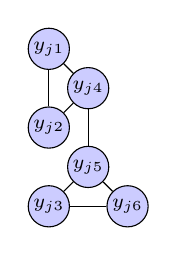
\begin{tikzpicture}[scale=1, main node/.style={circle, draw, fill=blue!20, inner sep=1pt, font=\scriptsize, minimum size=5mm, text=black}]
            % construction des triangles y_i
            \node[main node] (yj1) at (1, 0) {\(y_{j1}\)};
            \node[main node] (yj2) at (1, -1) {\(y_{j2}\)};
            \node[main node] (yj3) at (1, -2) {\(y_{j3}\)};
            \node[main node] (yj4) at (1.5, -0.5) {\(y_{j4}\)};
            \node[main node] (yj5) at (1.5, -1.5) {\(y_{j5}\)};
            \node[main node] (yj6) at (2, -2) {\(y_{j6}\)};
            
            % on connecte les y_i entre eux
            \draw (yj1) to (yj2);
            \draw (yj1) to (yj4);
            \draw (yj2) to (yj4);
            \draw (yj3) to (yj5);
            \draw (yj3) to (yj6);
            \draw (yj4) to (yj5);
            \draw (yj5) to (yj6);
        \end{tikzpicture}
    }
}